\documentclass[a4paper,html,11pt,openany]{book}
\usepackage{amsmath,mathtools}
\usepackage{longtable}
\usepackage{siunitx}
\usepackage{nicefrac}
\usepackage{listings}
\usepackage{color}
\usepackage{graphicx}
\usepackage{longtable}
\usepackage{ulem}
\usepackage{hyperref}
\definecolor{gray}{rgb}{0.4,0.4,0.4}
\definecolor{darkblue}{rgb}{0.0,0.0,0.6}
\definecolor{cyan}{rgb}{0.0,0.6,0.6}

\lstset{
  basicstyle=\ttfamily,
  columns=fullflexible,
  showstringspaces=false,
  commentstyle=\color{gray}\upshape
}

\lstdefinelanguage{XML}
{
  morestring=[b]",
  morestring=[s]{>}{<},
  morecomment=[s]{<?}{?>},
  stringstyle=\color{black},
  identifierstyle=\color{darkblue},
  keywordstyle=\color{cyan},
  morekeywords={xmlns,version,type}% list your attributes here
}
\usepackage{footnote}
\makesavenoteenv{tabular}
\begin{document}
  \title{Reference for the XML-Files for GOAT}
  \author{Thomas Weigel\\Applied Laser Technologies, Ruhr-Universit\"at Bochum, Germany}
  \date{\today}
  \maketitle
  \tableofcontents   
  \chapter{Introduction}
A calculation can be carried out directly via the GOAT library. Sometimes it is useful to save the scene information externally. A separate GOAT::XML::xmlReader class is available for this purpose. It is based on an XML file, the structure of which is described in more detail in this documentation. 
  In the following, we will given an overview on the structure of a XML file, which can be used as an input for the setup of the scene and for a couple of different calculation processes. Firstly, the principle structure will be discussed. Please note that all lengths are given in \si{\micro\metre}. After the usual preamble of the XML file, everything is encapsulated in the Root entry, i.e. $<$Root$>...<$\textbackslash Root$>$.   
   In the following, the term "section" is used for a closed part which is encapulated by $<$Sectionname$>...<$\textbackslash Sectionname$>$. Within the root section, there are two possible subsections, the Scene section, which describes the whole structure of the scene with all light sources, objects etc. and the calculation section where the calculation parameters are described. As values there are strings, integer or floating point numbers, threedimensional vectors and complex numbers. \textbf{Threedimensional vectors} are given by the x,y and z component. In the following sections, the parameters that apply equally to all elements of the same type (light sources, detectors, etc.) are specified first. Then only the specific parameters are specified.  \\
   examples: \\   

 \textbf{Threedimensional Vector}:   
    \lstset{language=XML}
 \begin{lstlisting}
 <position x="2.3" y="4.5" z="-5.6" />
   \end{lstlisting}
   A \textbf{complex number} is given its real and its imaginary part: 
 \begin{lstlisting}
 <n real="1.5" imag="0.1"/>
   \end{lstlisting}
  The default values for the threedimensional vector is (0,0,0) and for the complex number (0,0) unless otherwise specified. 
  Naming convention: The name of all elements which have childs like light sources, objects also position and direction etc. start with uppercase letters. In case a name consists of more than one word (like "numRays" for number of rays) the subsequent words start with uppercase letters. 
   
 \chapter{Scene}
 Within this section, all elements like light sources, objects and detectors are described. The scene has the following parameters: the radius of the calculation space r0.
 
  \vspace{1em}
 \textbf{Parameters used for all light sources} \\
 
 \begin{tabular}{c|m{3cm}|c|c}
 Parameter name & description  & possible value & default value\\ 
 \hline
 r0 & Radius of the calculation space & integer number & 1000 \\
 \hline
 nCellsPerDir & Number of cells per direction & integer number & 1000 \\
 \hline 
    \end{tabular} 
 \section{Light sources}
 All light sources have some entries which are used for all types. All parameters are optional. If one parameter is missing, it will be set to its default value, which is given in a table below. \\
 \vspace{1em}
 \textbf{Parameters used for all light sources} \\
 \begin{tabular}{c|m{3cm}|c|c}
 Parameter name & description  & possible value & default value\\ 
 \hline
 type & type of the light source & \parbox{5cm}{"plane","gaussian","ring",\\"tophat","plane\_mc",\\"gaussian\_mc","ring\_mc",\\"gaussian\_ring\_mc"} & -- \\
 \hline
 position & \parbox{3cm}{position of the light source\\(center of the area)} & 3D vector & (0,0,0) \\
 \hline
 NumRays & \parbox{3cm}{Number of rays per calculation step} & integer number & 100 \\
 \hline
 NumRaysRT & \parbox{3cm}{Number of rays for ray representation} & integer number & 10 \\
 \hline
wavelength\footnote{For pulsed calculation, this wavelength will be overwritten} & Wavelength of the light source &  floating point number & 1.0 \\
\hline
Polarisation & Polarisation & 3D Vector & (1,0,0) 
 \end{tabular}
 
 \vspace{1em} 
 Note: As described in more detail in the documentation for the LightSrc class, the polarisation here also refers to the case where the light source points in the z direction. The polarisation is rotated according to the direction defined in “Direction”. 
  \subsection{Plane wave}
  type: \textbf{plane} \\
 This type is the most simplest type of light source. This is a plane wave in which the rays are emitted equally distributed. The number of rays here only refers to one direction, i.e. the total number of rays is the square ($Numrays^2$). The distance between two adjacent rays is $\nicefrac{size}{numRays}$. The only special parameter is
  
\vspace{1em} 
  \begin{tabular}{c|c|c|c}
 Parameter name & description  & possible value & Default value \\
 \hline
 Direction & Direction of the plane wave & 3D Vector  & (0,0,1)\\
  \hline
  size & width of the light source  & floating point number & 10.0\\
 \end{tabular}
 
 \subsection{Plane wave (mc)} 
 type: \textbf{plane\_mc} \\
 All light sources denoted with "mc" are those where the rays are arbitrarily distributed. Unlike in the case of the plane wave, the total number of rays is equal to numRays. Also here, the only special parameters are "Direction" and "size". 
 
\subsection{Gaussian wave}
 type: \textbf{gaussian} \\
A gaussian wave describe a wave which is focused  towards the focal point and has a gaussian radial intensity distribution. The direction of the wave is given by the position of the light source and the focal point. For the description of the gaussian distribution, one can either give the (virtual) waist width at the focal point, w0 or the numerical aperture NA. If both are given, the numerical aperture is used. Please note, that the width (full width at half maximum) refers to the electric field: \\ 

\begin{align}
E&=E_0 \cdot e^{\frac{-x^2}{2\sigma^2}} \Rightarrow \sigma^2=\frac{\delta x_E^2}{8\ln2} \\
I&=I_0 \cdot e^{\frac{-2x^2}{2\sigma^2}} \\
\Aboxed {\delta x_I&=\frac{\delta x_E}{\sqrt{2}}}
\end{align}
with the width of the electric field $\delta x_E$ and the corresponding width of the intensity profile $\delta_I$.
\vspace{1em}
Special parameters:

\vspace{1em}
 \begin{tabular}{c|c|c|c}
 Parameter name & description  & possible value & default value\\
 \hline
 FocusPosition & Position of the focal point & 3D Vector & (0,0,0) \\
 \hline
 w0 & (virtual) waist at the focal point & floating point number & 1.0 \\
 \hline
 NA\footnote{if w0 and NA are given, NA is used} & numerical aperture & floating point number & 1.0 \\ 
   \hline
  size & width of the light source  & floating point number & 10.0
 \end{tabular}

\subsection{Gaussian wave (mc)} 
 type: \textbf{gaussian\_mc} \\
The same as the normal gaussian wave, except that the distribution of the rays is arbitrary and the intensity distribution is given by the density of the rays. 

\subsection{Ring shaped light source}
type: \textbf{ring} \\
A light source, shaped like a ring with equally distributed rays. The ring is described by its inner and outer radius. 

\vspace{1em}
 \begin{tabular}{c|c|c|c}
 Parameter name & description  & possible value & default value\\
 \hline
  rmin & inner radius ($\ge 0$) & floating point number & 0 \\
  \hline
  rmax & outer radius  & floating point number & 100 \\
  \hline 
  Direction & direction of the light rays & 3D vector & (0,0,1) \\
    \hline
  size & width of the light source  & floating point number & 10.0\\

\end{tabular} 
 
\subsection{Ring shaped light source (mc)}
 type: \textbf{ring\_mc} \\
Like ring shaped light source, except that the rays are distributed arbitrarily. 
 \subsection{Gaussian ring shaped light source (mc)}
type: \textbf{gaussian\_ring\_mc}
The light source consists of a Gaussian beam profile from which a ring is cut out. In contrast to the Gaussian beam, the rays are aligned in parallel.
Like all light sources denoted with "mc", the rays are distributed arbitrarily. The intensity is given by the density of the rays. 

\vspace{1em}
 \begin{tabular}{c|c|c|c}
 Parameter name & description  & possible value & default value\\
 \hline
 rmin  & inner radius & double ($0\le$ rmax) & 0 \\
 \hline 
 rmax & outer radius & double & 100 \\
 \hline 
 width & FWHM & double & rmax (100) \\
 \hline
 Direction & direction of the beam & 3D-Vector & (0,0,1) \\ 
\end{tabular}
 
\vspace{1em} 
 \textbf{Example for a scene with one light source}
 \lstset{language=XML}
 \begin{lstlisting}
  <?xml version="1.0" encoding="utf-8"?>
<Root>
  <Scene r0="4E+4">
    <nS imag="0.0" real="1.0" />
    <LightSources>
      <LightSource numRays="100000" size="1500" Type="ring_mc"
       wavelength="1.0"
       rmax="500" rmin="0">
        <position x="0.0" y="0" z="-1E+4" />
        <Direction x="0.0" y="0" z="1" />
      </LightSource>
    </LightSources>
 </Root>
 \end{lstlisting}
 Beside these general parameters, every type of light sources have there own special parameters

\subsection{Line shaped light source}
For some calculations a twodimensional calculation is sufficient. For this purpose a line shaped light source is introduced. Beside the position, this source is defined by its direction, which gives the direction of the rays and the orientation (lateral direction). 

 \section{Objects}
 Like the light sources, all objects have some general parameters. Those parameters can be seen in the following table
 
 \vspace{1em}
% \begin{tabular}{c|c|c}
 \begin{longtable}{p{2cm}|m{3.5cm}|m{3.0cm}|p{1.7cm}}
 Parameter name & description  & possible value & default value\\
 \hline
  Position & Position of the object\footnote{Reference point for the object differ from shape to shape} & 3D Vector & (0,0,0) \\
  \hline
  type & Type of the object  & \parbox{3cm}{ellipsoid,\\surface,\\cone,\\aspheric\_lens,\\box} & --  \\
  \hline   
  scaling & The object will be scaled by this factor & double & 1.0 \\
  \hline
  alpha & \parbox{3.5cm}{rotation angle\\around x-axis\\(in radiants)} & double & 0 \\ 
    \hline
  beta & \parbox{3.5cm}{rotation angle\\around y-axis\\(in radiants)} & double & 0 \\ 
      \hline
  gamma & \parbox{3.5cm}{rotation angle\\around z-axis\\(in radiants)} & double & 0 \\ 
  \hline
  isactive & \parbox{3.5cm}{Fields inside the object will be stored (this concerns e.g. the pulsed calculation and the inelastic scattering)} & true/false & false \\
  \hline
  n & refractive index & complex value & (1.0,0.0) 
\end{longtable} 
  
\subsection{Ellipsoid}
 type: \textbf {ellipsoid} \\
 This object type describes an elliptic object, defined by the three semi-axis, according to
  \begin{equation}
  \frac{(x-x_c)^2}{a_x^2}+\frac{(y-y_c)^2}{a_y^2}+\frac{(z-z_c)^2}{a_z^2}=1
\end{equation}   
The position is defined by the center of the ellipsoid ($x_c$,$y_c$,$z_c$).

\vspace{1em}
\begin{tabular}{p{2cm}|m{3.5cm}|m{3.0cm}|p{1.7cm}}
 Parameter  & description  & possible value & default value\\
 \hline
 Dimension & Vector which holds semi-axis along the x-, y- and z-direction & 3D Vector & (10,10,10) 
 \end{tabular}
%  \end{center}
 \subsection{Box}
 type: \textbf{box} \\
 This object type describes a cuboid, defined by the edge lengths. The center of the cuboid is used as position (reference point).
 
\vspace{1em} 
\begin{tabular}{p{2cm}|m{3.5cm}|m{3.0cm}|p{1.7cm}}
 Parameter  & description  & possible value & default value\\
 \hline
 Dimension & Vector which holds the edge lengths along the x-, y- and z-direction & 3D Vector & (10,10,10) 
 \end{tabular}
 
 \subsection{Cylinder}
 type: \textbf{cylinder}
 This object type is a spheric cylinder. 
 
\vspace{1em} 
\begin{tabular}{p{2cm}|m{3.5cm}|m{3.0cm}|p{1.7cm}}
 Parameter  & description  & possible value & default value\\
 \hline
height & Height of the cylinder & double & 1 \\
\hline
radius & Radius of the cylinder & double & 1 \\
\end{tabular}  
 
\subsection{Surface}
type: \textbf{surface} \\
A the surface of a surface object is described by triangles stored in a file. Up to now two file formats are supported:
\begin{itemize}
\item {\bf SRF}-files: A proprietary file format. The first entry is the number of triangles stored in the file, followed by a list of the triangles. This file format is described in more detail in the documentation of the GOAT library. 
\item {\bf STL}-files: Here only binary stl-files are supported. 
\end{itemize} 

 
\vspace{1em} 
\begin{tabular}{p{2cm}|m{3.5cm}|m{3.0cm}|p{1.7cm}}
 Parameter  & description  & possible value & default value\\
 \hline
 filetype & String, which holds the file type & ".srf",".stl" & -- \\
 filename & String, which holds the file name & string & -- \\
 \end{tabular}
 
\subsection{Spheric lens}
type: \textbf{spheric\_lens} \\
A spheric lens is described by the two side faces (see also documentation of the GOAT-library for details). It has two child elements named "left" and "right" for the two corresponding surfaces. 

 
\vspace{1em} 
\begin{tabular}{p{2cm}|m{2cm}|m{2.5cm}|m{2.0cm}|p{1.7cm}}
 subcategory  & parameter & description  & possible value & default value\\
 \hline
 & radius  & radius of the lens (cross section) & double & 0 \\
 \hline
 & offset & offset between the sides & double & 0 \\
 \hline
 left(right)\footnote{parameters for the subcategories "left" and "right" are the same} & & Subcategory for the left(right) side & N/A & N/A  \\
 \hline
  left(right) & Curvature & Curvature type & "flat", "concave" or "flat" & --  \\
    left(right) & R & Radius  & convex, concave, flat (enumerator)  & flat  \\
 \end{tabular}
 
\subsection{Vortex phase plate}
type: \textbf{vortex\_plate} \\
A vortex phase plate as shown in Fig.\ref{fig:vortexplate} is an object to create a vortex beam. It is defined by its height $dh$ and the topological charge $m$, which gives the number of subdivisions. The full object is described by a cylinder with a given height and on top,the spiral vortex structure.   
\begin{figure}[h!]
   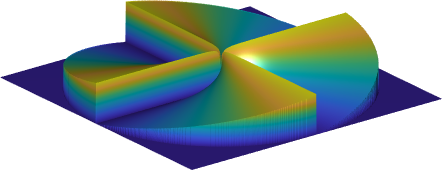
\includegraphics{vortex_plate.png}
   \caption{Vortex phase plate with $m=4$}
   \label{fig:vortexplate}
\end{figure} 

\vspace{1em}
\begin{tabular}{p{2cm}|m{3.5cm}|m{3.0cm}|p{1.7cm}}
 Parameter  & description  & possible value & default value\\
 \hline
 height & height of the base cylinder & double & 1 \\
 \hline
 radius & radius of the object & double & 1 \\
 \hline
 m & topological charge & integer & 1\\
 \hline
 dh & height of the vortex & double & 1 \\
 \end{tabular}
 
 \section{Detectors}
 A detector is a special twodimensional object in which the electric field is stored. Like for the light sources and the objects the section is encapsulated in a tag with sectioname "Detectors". 
  
 \vspace{1em} 
\begin{tabular}{p{2cm}|m{3.5cm}|m{3.0cm}|p{1.7cm}}
 Parameter  & description  & possible value & default value\\
 \hline 
 type & type of the detector & "plane" & -- \\
 \hline
 Position & Center of the detector & 3D-vector & -- \\
 \hline
 Direction & normal vector & 3D-vector & -- \\
 \hline  
 filename & name of the file to store the data & string & -- \\
  \end{tabular}
  
 \subsection{Plane detector}
 type: \textbf{plane}
 This is square plane detector object. \newline
 Special parameters: 
 
 \vspace{1em} 
\begin{tabular}{p{2cm}|m{3.5cm}|m{3.0cm}|p{1.7cm}}
 Parameter  & description  & possible value & default value\\
 \hline 
d & width of the detector & double & 1 \\
\hline
n & no. of elements per direction & int & 1 \\ 
\end{tabular}
 
 \chapter {Calculations}
 Also, calculations can be defined and started with help of the XML file. Calculations are given in the section "Calculations". Similar to the definition of the light sources, every single entry for a calculation starts with "Calculation". Depending on the attribute "type" there are different calculations possible:
 
 %\begin{center}
 \vspace{1em}
 \begin{tabular}{c|m{8cm}}
 type name & description \\
 \hline
 pure & Raytracing will be done without any further calculation will be done. Only detectors are considered.\\
 \hline 
 path & Raytracing will be performed, path of the rays can be stored in a file. \\
  \hline
 pulse & Calculation with pulsed light source will be performed.
 \end{tabular}
% \end{center}
 
 \vspace{1em}

 Parameters for all calculations
 \begin{table}[h!]
\fontsize{10pt}{10pt}\selectfont
 \begin{tabular}{c|m{3cm}|m{3cm}|c}
  Parameter name & description  & possible value & default value \\
 \hline
 type & type of the calculation & \parbox{3cm}{"pure","path",\\"pulse"} & -- \\
 \hline
 inactive & if true, this calculation will be skipped & true, false & false \\
 \hline 
 \end{tabular}
 \end{table}

\section{Calculation with detectors only}
If one want only the electric field distribution at certain areas, this calculation type "\textbf{pure}" is the right choice. Here, beside light sources and objects, only the detectors will be considered. Therefore no further special parameters are needed. 
 \section{Calculation of the ray paths}
 Sometimes it is necessary to know the path of the rays through the scene. This can be done with the calculation type "{\bf path}". In the file, the starting and ending positions of each step, i.e. from surface to surface (or from light source to surface).
 The corresponding parameters are
 
 \vspace{1em}
 \begin{table}[h!]
\fontsize{10pt}{10pt}\selectfont
 \begin{tabular}{c|m{3cm}|m{3cm}|c}
  Parameter name & description  & possible value & default value \\
 \hline
 filename & Name of the file in which the paths are stored. This parameter is essential & string & -- \\
 \hline 
 numRays & Number of rays\footnote{The meaning of this parameter depends on the type of source} & integer & 1 \\
 \hline 
 numReflex & Number of reflections & integer & 0 \\
 \hline 
 \end{tabular}
   \end{table}
   Sometimes it is convenient to switch off calculations without erasing it. For this reason, the property "inactive" can be set to "true". ´ 
 \section{Calculations with pulsed laser sources}
 Here, all light sources are considered as mode-locked lasers.  For this calculation, two different methods for the Fourier transform can be applied. On the one hand, a pure raytracing calculation can be performed, here attribute "Method" is set to "rtonly". On the other hand a mixture of raytracing and an integral can be used (attribute "Method" is not set). Here, the frequency range used for the calculation is divided into frequency divisions. For each division, one raytracing at the center frequency is performed. Here a gaussian pulse shape is considered. As parameter the pulse width $\Delta t$(FWHM of the intensity profile) in \si{\femto\second} can be given. The corresponding spectral width (FWHM) $\delta \omega$ is directly connected with $\Delta t$ by
 \begin{equation}
  \delta \omega=\frac{4\cdot\ln 2}{\delta t}.
 \end{equation}
 To get a better result of the pulse, a spectral width $\Delta \omega = 5 \cdot \delta \omega$ is used. The distance between two subsequent pulses $\tau$ is then given by
 \begin{equation}
   \tau=\frac{2\pi N}{\Delta \omega}
 \end{equation}
The parameters are as follows: 
 \vspace{1em}
 \begin{longtable}{c|m{3cm}|m{3cm}|c}
\fontsize{10pt}{10pt}\selectfont
% \begin{tabular}{c|m{3cm}|m{3cm}|c}
  Parameter name & description  & possible value & default value \\
 \hline
 \tiny{estimateTimeForObject} & The time when the pulse hits the object with the given number. This can only be used with one light source. If a time is given, it is relative to this estimated time. Can only be used without method "rtonly"! & number of the corresponding object & -- \\
 \hline
 time & Time at which the fields are calculated & -- \\
 \hline
  filename & \parbox{3cm}{Prefix of the filename used to store the result. A file for each active object will be created in the form $<$filename$><$object no.$>$.dat}. & any filename & -- \\
  \hline
  spatialResolution & resolution of the grid in \si{\micro\metre} & double $>0$ & 1 \\
  %$\frac{2\cdot r_0}{nn\footnote{number of elements per direction}}$
  \hline 
  wavelength & Central wavelength in µm & double & $\SI{1}{\micro\metre}$ \\
  \hline
  numReflex & Number of reflections & integer $\ge$ 0 & \tiny{INEL\_MAX\_NREFLEX (1)} \\
  \hline
  numLoops & Specifies how often the calculation should be repeated (-1: calculation is repeated infinitely often) & integer $\ge$-1 & -1 \\
  \hline
  pulseWidth & \parbox{3cm}{Pulse width \\ (FWHM)  in \si{\femto\second} }& double & \SI{100}{\femto\second} \\
  \hline
  method & \parbox{3cm}{For the calculation a pure raytracing calculation will be performed (the fields for all wavelengths will be calculated by raytracing) or a mixed method can be applied} & "rtonly","mixed" & "mixed" \\
  \hline
  numSpectralRanges & Number of spectral ranges considered for calculation & integer $\ge$ 1 & 4 \\
  \hline 
  RefractiveIndexList & List of the refractive indices of the materials & see below & N/A \\   
% \end{tabular}
 \end{longtable}
 The refractive index list is organized as follows: \\
 For the objects, the corresponding attribute is named as "n0" for the first object, "n1" for the second and so on. The order is given by the order in which the objects are defined in the objects-section. The attribute for the surrounding medium is "nS". Possible values are given in Table \ref{tab:refractiveIndexList}. 
 
 \vspace{1em}
 \begin{center}
 \begin{table}
 \begin{tabular}[H]{l|l}
 Material & value \\
 \hline 
 Air & air \\
 Glass & glass (allways refractive index 1.5) \\
 N-BK7 glass & bk7 \\
 N-LASF55 glass & lasf55 \\
 Vacuum & vacuum \\ 
 PMMA & pmma \\
 \end{tabular}  
 \caption{List of the possible values for the refractive index list}
 \label{tab:refractiveIndexList}
\end{table}
 \end{center}
 For vacuum and glass constant refractive indices were used (1 for vacuum and 1.5 for glass). The other dispersion curves were taken from \url{https://www.refractiveindex.info}. 
\end{document}
